\chapter{Background Theory}
\label{BackgroundTheory}
\graphicspath{{Figures/BackgroundTheory/}{Figures/Common/}}

\section{Absorbing boundary layers for Schrödinger-type equations}
\label{BackgroundTheory:AbsorbingBoundaryLayers}


To solve any partial differential equation numerically, it must be restricted to a finite domain with boundary conditions imposed at the edges\footnote{This requirement can be avoided when the solution's asymptotic behaviour is known \emph{a priori}, however this case will not be encountered in this thesis.}. For some systems, this poses no additional restriction over the original problem as they are explicitly defined over a finite domain and with the correct boundary conditions this constitutes the problem itself (for example electromagnetic wave propagation in a waveguide). Other systems are naturally restricted to a finite domain (for example a BEC in a trap) and will be unaffected by the imposition of the artificial boundary conditions. 

With the exception of systems defined over a finite domain, the choice of boundary conditions at the edges of the computational domain is an artificial one; while in many cases they permit physical interpretation, this interpretation does not usually correspond to the reality of the system under consideration. A strategy is therefore needed to limit the effect of the choice of boundary conditions on the solution.  In some cases the solution is naturally restricted to a finite domain (e.g. a BEC in a harmonic trap) and is unaffected by the choice of boundary conditions.  This is not always the case, the Gross-Pitaevskii equations for an atom laser are naturally defined on a semi-infinite domain to accommodate the motion of the atom laser. These equations will be considered extensively in this thesis and a strategy must be used to prevent the moving atom laser beam interacting with the artificial boundary conditions.

A first simple strategy would be to choose the computational domain to be large enough such that no part of the atom laser beam will reach the edge of the domain over the time of interest. While effective, this strategy can be computationally expensive and is particularly demanding in the presence of gravity. Under the influence of gravity a classical particle starting from rest will travel a distance $d = \frac{1}{2}g t^2$ in time $t$. Hence the size of the computational domain must increase as $t^2$. The spatial grid separation cannot remain constant however. As the velocity of the classical particle increases as $v = gt$, the mean wavelength of the particle $\displaystyle \lambda = \frac{\hbar}{Mv}$ must then decrease as $t^{-1}$.  To resolve the spatial dynamics of the atom laser, the step size between points must then decrease as $t^{-1}$. These two effects combine to give the scaling that the total number of spatial grid points required $N_\text{pts} \propto t^3$. Choices of uniform or variable spacing for the grid will only differ by an overall constant factor in the number of points required by this strategy; such choices cannot change the overall scaling. A different strategy is needed.

In many circumstances it is the Bose-Einstein condensate and the outcoupling process that produces the atom laser that are of interest. In such situations the remainder of the atom laser that can no longer directly interact with the BEC must be prevented from doing so as a result of its unphysical interactions with the artificial boundary conditions. The solution used in the aforementioned strategy was to continue to model the atom laser, however this is not necessary. An alternative solution is to remove this part of the atom laser from the simulation in a way that has no effect on the BEC and the outcoupling process. One strategy that takes this approach is to add an \emph{absorbing boundary layer} \citep{Kosloff:1986,Neuhasuer:1989} between the domain of interest and the artificial boundary conditions. This absorbing boundary layer takes the form of a negative imaginary potential, which must be chosen to be deep enough to strongly attenuate any wave traversing it and smooth enough to make the probability of reflection negligible. \figureref{BackgroundTheory:AbsorbingBoundarySchematic} illustrates this strategy.

\begin{figure}
    \centering
    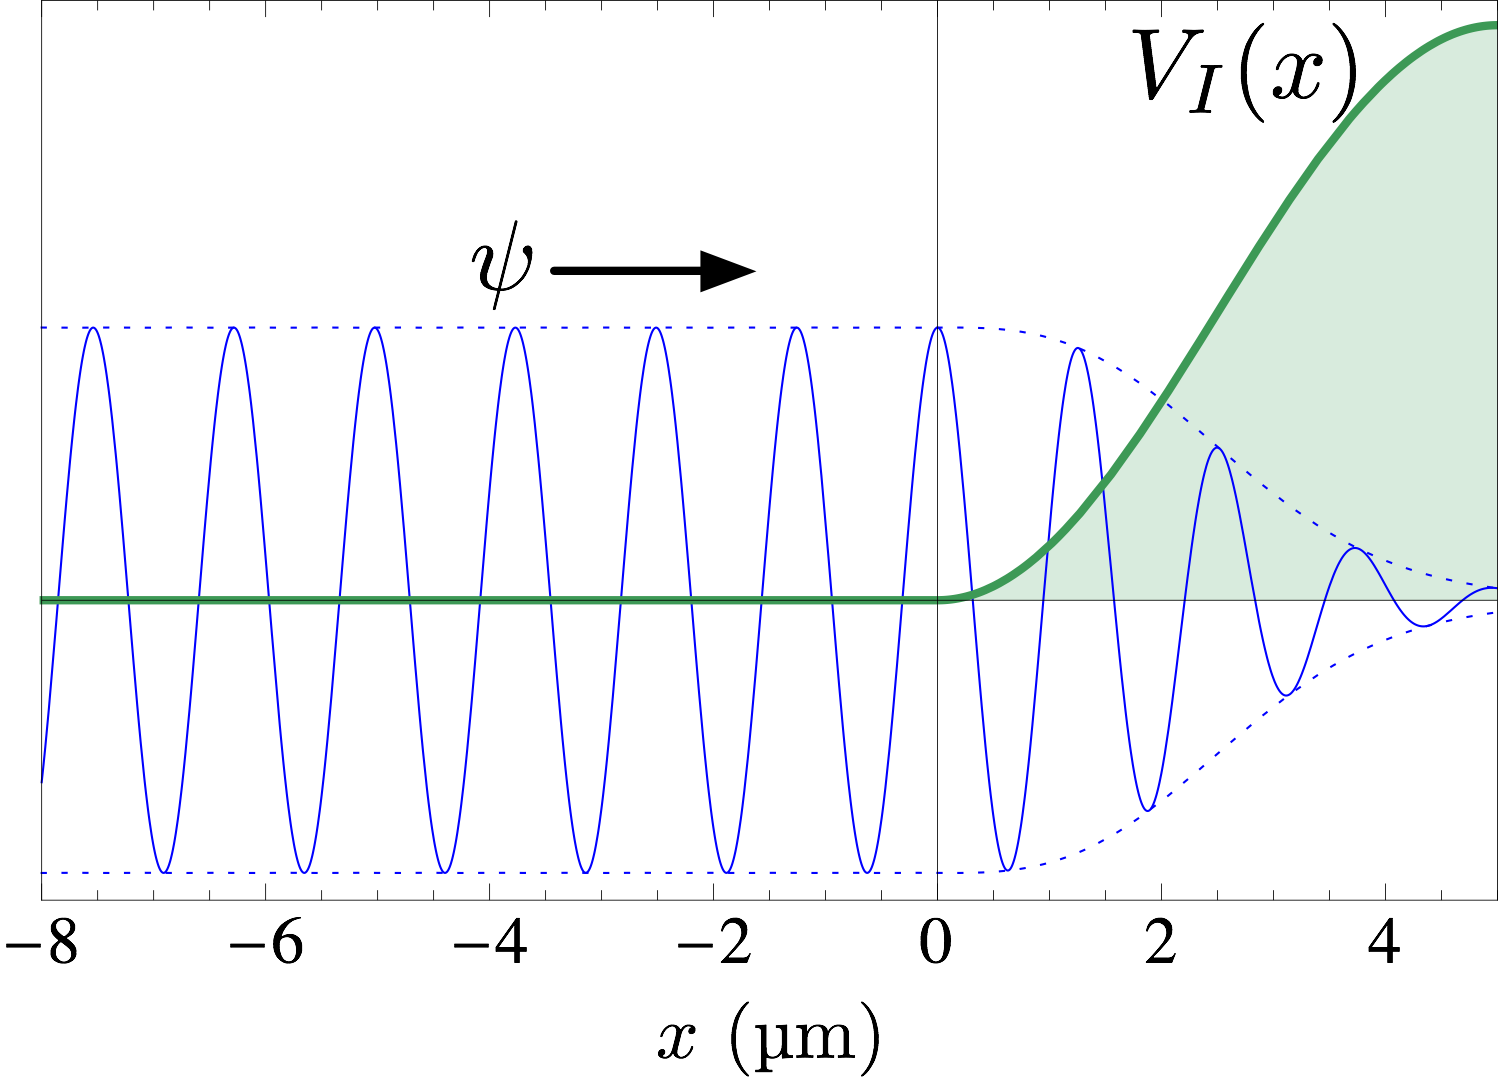
\includegraphics[width=8cm]{AbsorbingBoundarySchematic}
    \caption{
        \label{BackgroundTheory:AbsorbingBoundarySchematic}
        Schematic diagram illustrating the use of an absorbing boundary layer. A right-travelling wave is incident on the absorbing boundary layer which is given by the potential $V(x) = -i V_I(x)$. The wave is attenuated as it crosses the absorbing boundary layer.
    }
\end{figure}

An absorbing boundary layer of finite thickness can only be effective over a finite range of incident wavenumbers. Incident wavefunctions with large wavelengths (low wavenumbers) will be reflected from the absorbing boundary layer due to the rapid change in the potential over a wavelength. Incident wavenumbers with very short wavelengths (high wavenumbers) will be transmitted through the absorbing boundary layer due to the finite amount of time spent in the absorbing boundary layer by any given point on the phase-front.  Using this argument \citet{Neuhasuer:1989} showed that the approximate range of wavenumbers over which an absorbing boundary layer will be effective is
\begin{align}
    \label{BackgroundTheory:AbsorbingBoundaryKEffectiveRange}
    \left( \frac{M \overline{V_I}}{\hbar^2 \Delta x}\right)^{\frac{1}{3}} \ll k \ll \frac{2 M \overline{V_I} \Delta x}{\hbar^2},
\end{align}
where $\overline{V_I}$ is a representative value of $V_I(x)$. The limit on the maximum and minimum size of the wavenumber are respectively due to the requirements of negligible transmission and reflection. Although cast in terms of the wavenumber, \eqref{BackgroundTheory:AbsorbingBoundaryKEffectiveRange} is equivalent to (26) in \citep{Neuhasuer:1989}.

Using an argument derived from that given by \citet{Neuhasuer:1989}, the approximate range of wavenumbers over which the absorbing boundary layer will be effective can be quantified by considering an incident wave of wavenumber $k$ on a potential $V(x) = -i V_I(x)$ of finite width $\Delta x$. As it is the efficacy of the absorbing boundary layer that is under consideration, it will be assumed that the potential is zero everywhere. The results of these calculations will then apply in terms of the wavenumber of the wave as it is incident on the absorbing boundary layer provided the physical potential changes negligibly over the scale of the absorbing boundary layer. It will also be assumed that the mean-field interactions of the atom laser are small compared to the kinetic energy and can be neglected.\footnote{FIXME: Paragraph needs rewrite.}



In this thesis, the abstract boundary conditions used most frequently will be periodic boundary conditions due to the effectiveness of the Fast Fourier Transform (FFT) algorithm that permits efficient transformation between the position basis and the spectral basis.



A different strategy will be used in \chapterref{TransverseProfile} in which the spatial profile of the atom laser a large distance from the BEC is considered. In this situation the strategy discussed above cannot be used as it is precisely the behaviour of the atom laser far away from the BEC that is of interest. A third strategy that is appropriate for considering the behaviour of the atom laser far from the BEC is discussed in \sectionref{TransverseProfile:DropGP}.



The use of an absorbing boundary layer is an approximation; no finite layer can perfectly absorb any incident wave without causing reflections.

This argument is formalised in \citep{Neuhasuer:1989}.